% !TEX encoding = UTF-8 Unicode
\documentclass[]{uvamscse}
\usepackage[square, numbers, comma]{natbib}
\usepackage{nameref}
\usepackage{url}
\usepackage[singlelinecheck=false]{caption}
\usepackage{verbatim}
%\usepackage[]{algorithm2e}

%% Draft section
\usepackage{draftwatermark}
\SetWatermarkText{-DRAFT-}
\SetWatermarkScale{5}

%% Add revision history page
\renewcommand{\revisionhistory}{
	\newpage
	\chapter*{Revision history}

\begin{tabular}{p{2cm} p{7cm} p{5cm}}
	\hline
	\bfseries{Version}\rm & \bfseries{Recipients}\rm & \bfseries{Remarks}\rm \\
	\hline
	20140324 & ir. Rutger Pannekoek & draft Introduction, Method \\
	20140410 & dr. Magiel Bruntink, ir. Rutger Pannekoek & draft Introduction,
	Method, Research
	\\
	20140611 & dr. Magiel Bruntink, ir. Rutger Pannekoek & for review \\
	20140712 & dr. Magiel Bruntink, ir. Rutger Pannekoek & published \\
	\hline
\end{tabular}

	\newpage
}
%% end Draft section

\makeatletter
\let\orgdescriptionlabel\descriptionlabel
\renewcommand*{\descriptionlabel}[1]{%
	\let\orglabel\label
	\let\label\@gobble
	\phantomsection
	\edef\@currentlabel{#1}%
	%\edef\@currentlabelname{#1}%
	\let\label\orglabel
	\orgdescriptionlabel{#1}%
}
\makeatother

\renewcommand{\arraystretch}{1.5}
\newcommand{\keywords}{\vspace{1cm}\noindent\bfseries{Keywords: }\rm}

% research hypothesis and questions
\newcommand{\researchQuestion}{Can we use wavelet analysis to find objective
warning signs in OSS projects leading to the end of code evolution?}
\newcommand{\subQuestionOne}{What patterns can be found using wavelet analysis?}
\newcommand{\subQuestionTwo}{Under what conditions does wavelet analysis
succeed or fail in detecting evolutionary events?}

% title section
\title{Automatic Means of Detecting Warning Signs in Software Evolution}
\author{ing. Martijn Endenburg}
\authemail{martijn.endenburg@gmail.com}
\host{VNU Vacature Media \emph{division of De Persgroep Nederland}\rm}
\newcommand{\hostOrg}{VNU Vacature Media}
\supervisor{dr. Magiel Bruntink (UvA), ir. Rutger Pannekoek (VNU)}
\docstatus{Draft}

\abstract{
	\em
Abstract here

\rm
\smallskip
\noindent \textbf{Keywords:} keywords, here

}

\begin{document}
\maketitle

%% Keep table resize here to make only tables inside the text smaller font
\let\oldtabular\tabular
\renewcommand{\tabular}{\footnotesize\oldtabular}
\renewcommand{\thetable}{\Roman{table}}
%% /Table

This thesis is the result of my graduation project. I started the project in
January 2014 and finished it in July 2014, a total track of 7 months of
iteratively planning, performing, observing, analysing, and writing. It
concludes the part-time Master programme Software Engineering at the University
of Amsterdam, The Netherlands.

The project has been performed at VNU Vacature Media, the company at which I am
employed at. VNU Vacature Media, since May 2012 a division of De Persgroep
Nederland, operates in the on-line recruitment market. It serves the largest
job boards in The Netherlands and Belgium, such as Intermediair, Nationale
Vacaturebank, Vacature.com, and References.be. The software supporting these
products are mostly open-source, that is why the evolution of open-source
software came to my interest for choosing this subject.

\section*{Acknowledgements}
There are some people I would like to thank that contributed to my project
in various ways. This thesis would not have been possible without them.

\paragraph{}
First, I would like to thank Brett Kelly, who was CTO at VNU Vacature Media at
the time I started the Master's programme, and Rutger Pannekoek, who is CTO of
VNU Vacature Media since 2013. Without them, I wouldn't be able to follow the
Master's programme together with my job in the first place.

Then, I would like to thank my colleagues Bas,
Boudewijn,
Danny,
Eugene,
Ewout,
Greg,
Hugo,
Jan-Willem,
Jeroen,
Jerry,
Joeri,
Johan,
Marc,
Marvin,
Merlijn,
Michiel,
Nienke,
Kalle,
Leonard,
Tim,
and Wouter (I am sorry if I forget anyone, but this counts for you too), you
were all great in supporting me and my research on the days that I was
physically present, but mentally absent.

I would also like to thank my parents, Johan and Carla Endenburg, who supported
me and taught me that ``when there's a will, there's a way''.

Additionally, I would like to thank Siim Karus for helping me replicating his
research. He has been very helpful, especially in the beginning of the project,
in providing me his scripts and insights in his data.

Last, but definitely not least, big thanks to my girlfriend Christine
Fr\"{o}ger, for all the love, support, patience, and encouragements to complete
this thesis and to take breaks too every now and then.\\[2em]

\noindent
Martijn Endenburg\\
Amsterdam, \today


\chapter{Introduction}
\label{introduction}

This chapter introduces the research topic by describing the problem the
research is aiming to solve, and the motivation for the research direction.

\section{Problem statement}
Many elements of the software development process are related to the project's
progress. These elements include, but are not limited to, team composition,
team size, frequency of releases, developer's activity, and developer's and
user satisfaction \cite{crowston2006, delone1992, samoladas2010}.

A change in one or more of these elements affects the project's progress
positively or negatively. If a change in one or more of the elements has a
substantial effect on the project's progress, we call it an \emph{evolutionary
event}\rm; an event that changed the project's evolution.

\paragraph{}
In closed source projects, many evolutionary events are the effect of decisions
made by the management. The majority of closed source software projects are
initiated and maintained by commercial organisations. These projects evolve
according to changing business requirements, strategies, and commercial goals.

In commercial organisations, a change in the hiring policy, or planning and
deadlines, can become an evolutionary event for the projects affected by these
changes. These events can be used to identify project scale and progress. This
allows comparing and co-analysing different projects \cite{karus2013}.

\paragraph{}
In open-source software (OSS) projects, evolutionary events are mostly
theoretical with little empirical validation. Changes in development activity,
community, and other aspects of the OSS process are mostly organic. A community
of an OSS project changes continuously, often with little impact on the
evolution of the project \cite{androutsellis}. This means that different OSS
projects cannot be compared on the same scale. In other words, different OSS
projects cannot be objectively assessed by their evolution data without a
proper transformation of that data.

\paragraph{}
For closed source projects, the measurement of a project's success or
effectiveness is critical to our understanding of the value and efficacy of
management actions and investments \cite{delone2003}.

Comparing and analysing OSS projects is of interest to better understand the
survivability of OSS projects. The key factors that define the success or
failure of an OSS project have not yet been found.

\paragraph{}
We expect to be able to find indicators of failure in the events that
shape a project's evolution. Therefore, a means to identify these evolutionary
events would be useful. For closed-source software projects in a commercial
environment, these events can be easily tracked by the managerial history of
the project. For OSS projects, this is not the case.



\section{Motivation}
At \hostOrg, developers extensively use OSS projects in their day-to-day
work. The projects vary from developers tools, and utilities, to operating
systems and full system stacks. These OSS projects include, but are not limited
to, Ansible, Apache Web Server, MySQL, OpenStack, OpenVPN, and Ubuntu/Linux.
Besides the previously listed well-known projects, lesser known projects are
also used.

\paragraph{}
Given that OSS projects are popular in many organisations, and, as a result,
OSS projects contribute to the overall value of the products and services of
these organisations, a means to objectively assess OSS project's survivability
is of value. An assessment of the survivability of an OSS project will aid in
the decision for selection and/or continuity of a project.

\paragraph{}
In the study \emph{Automatic Means of Identifying Evolutionary Events in
Software Development }\rm by \citet{karus2013}, \citeauthor{karus2013} proposed
the use of wavelet analysis to automatically detect anomalies in OSS projects.

\paragraph{}
Wavelet analysis is used in many fields having many purposes. One of the
applications of wavelet analysis is pattern recognition in digital signal
processing, such as duplication detection and face recognition in imagery
\cite{myna, wadkar}. The wavelet algorithms process data at different scales or
resolutions \cite{graps}. The big advantage of wavelet analysis is that we are
able to analyse the data at different scale levels. Another advantage is that it
is based upon mathematical principles, making it fairly easy to automate.

\paragraph{}
At first glance, it may seem odd to use wavelet analysis to analyse evolution of
software projects. Software evolution data comprises various metrics, such as
lines of code, number of developers, number of commits, etc. The measures of
these metrics are all snapshots of moments in time. These metrics can be
modeled in the frequency domain of a waveform. The metrics have a functional
relation to the age of a project, which fits the time domain of a waveform.
This gives a natural transition of each metric to be modeled as a waveform and
enables the analysis of such a waveform.

\paragraph{}
When analysing waveforms of software evolution metrics, we should be able to
detect anomalies in these waveforms. After investigating and comparing these
anomalies we might as well be able to find the patterns that resulted from
evolutionary events. A comparison with known events that had a negative effect
on a project's progress may reveal that we are able to detect warning signs in
software evolution.\\

\noindent
According to \citet{karus2013}, knowing these warning signs will help in:
\begin{itemize}
	\item Choosing an OSS project to implement in a business scenario.
	\item Making timely preparations for decommissioning an OSS project.
	\item Choosing a development process that best suits the aims of a software
	project for new OSS projects.
\end{itemize}

\subsection{Warning sign}
A warning sign is defined as any pattern in the waveform that has a high chance
of resulting in the \emph{end of code evolution }\rm of a project. The
\emph{end of code evolution }\rm means that the source code activities of a
project have stopped. There could still be commits on the project, for instance
in Wiki pages, external library updates, or documentation, but no more source
code changes. For a pattern being such a warning sign, it has to be similar to
patterns that are confirmed to be such warning signs.



\section{Research questions}
\label{questions}

\begin{description}
	\item[RQ1\label{itm:question_warningsigns}]
	\emph{\researchQuestion}\\[0.3cm]
\end{description}

\noindent
In order to find the answer to the main question, the following
questions will be answered:
\begin{description}
	\item[RQ2\label{itm:question_patterns}] \emph{\subQuestionOne}
	\item[RQ3\label{itm:question_successfailure}] \emph{\subQuestionTwo}
\end{description}

\paragraph{}
We are not looking for OSS vitality as the project's ability to provide support
and grow in the number of releases. In this study, we only look at the
development process using software analytics, ignoring documentation and
community support.

\section{Outline}

Chapter \ref{background} will provide more information on prior research in the
field of OSS project survivability. In chapter \ref{method} the method and
approach of the research is discussed. Chapter \ref{research} describes the
research execution. In chapter \ref{results}, the results are presented, and
chapter \ref{analysis} provides the results after analysis and presents the
conclusions of the research.

\begin{comment}

INTRODUCTION

An introduction and overview of your thesis. Be sure to structure your thesis
such that you do not have to repeat yourself later. In this section you do not
cover details, but you give the reader an idea of the context, a brief overview
of the research, and how the remainder of the thesis is structured.


MOTIVATION

This section describes in detail what problem the research is addressing, and
what the motivation is to address this problem.

There is a concise and objective statement of the research questions (or
hypotheses you are testing) and goals. It is made clear why these questions and
goals are important and relevant to the outside world (i.e., the field of
research or industry that you are addressing). You can already split the main
research question into sub questions in this chapter.

This section also describes an analysis of the problem: where does it occur and
how, how often, and what are the consequences?

An important part is also to scope to research: what aspects are included and
what aspects are deliberately left out, and why? An example introduction can be
found on Paul Klint’s
homepage\footnote{http://homepages.cwi.nl/~paulk/thesesMasterSoftwareEngineering/2006/ReinierLabee.pdf}.
\end{comment}

\chapter{Research method}
\label{method}

This chapter elaborates on the steps to be taken in order to answer the
research questions. A description of each of the phases of the research is
given.

\section{Data selection}
\label{method:data}

The data for this research is provided by a tool by \citet{ohlohanalytics}.
This tool, ``\emph{OhlohAnalytics}\rm'', was developed as part of the
replicative research by \citet{bruntink2014}, and provides a validated and
cleansed data set of more than 10,000 OSS projects.

The projects are tracked by and gathered from Ohloh.net: \emph{``Ohloh is a
free, public directory of Free and Open Source Software and the contributors
who create and maintain it.'' }\rm \cite{ohloh}.

At the time of this writing, Ohloh tracks more than 660,000 OSS projects varying
in all ranges of size, and popularity. The most popular projects currently being
Apache HTTP Server, Apache OpenOffice, Apache Subversion, Bash, Firebug, Linux
Kernel, Mozilla Firefox, MySQL, PHP, and Ubuntu.

\subsection{Data validation and cleansing}
The OhlohAnalytics tool provides us with an initial data set of more than
10,000 OSS projects \cite{bruntink2014}. The raw data gathered from Ohloh
regularly contains errors and inconsistencies. This tool analyses the
consistency of the data and cleanses the data where needed. This results in a
consistent data set of project evolution data.



\subsection{Project selection criteria}

From the initial 10,000+ projects of which the evolution data is consistent, a
subset of 250 projects will be made. \citet{karus2013} used a data set of 27
projects to perform his wavelet analysis research. We believe a larger
data set will yield more trustworthy results. The number 250 is a somewhat
arbitrary number, but chosen to have a substantial larger set than the initial
study by \citeauthor{karus2013}, but still keep it feasible to analyse and
validate the data and results within the given time constaints of 4 months for
this thesis.

\subsubsection{Subsequent data series}
Prior to the selection of the projects for the study, another validation
step is needed. Although the set of 10,000+ projects' evolution data is
consistent, not all of it is suited for wavelet analysis.

To be able to perform wavelet analysis on any series of data, we need to have
a subsequent series (i.e., without gaps) of evolution data for each project
under study. Therefore, all the 10,000+ projects will be analysed for continuity
and only the projects that have a subsequent series of data are kept.

\subsubsection{Minimal sequence length}
A time series of 1 (monthly) data point is obviously not analysable over time
and uncomparable to larger projects. The threshold of at least 12 monthly data
points is chosen to minimise noise in the evolution data that may be caused by
too young and unstable projects.

\subsubsection{Representativeness}
Another criterion for the selection of projects in the data set is that they
form a subset that is representative to the set of all OSS projects tracked by
Ohloh.net. A tool created by \citet{nagappan} at Microsoft Research that is able
to determine the representativeness of a subset of projects will be used. This
tool scores projects by two metrics: total lines of code, and yearly
contributors count.

The tool by \citet{nagappan} is also capable of selecting a sample based on a
given baseline project and a total subset size. It keeps adding projects to the
subset as long as the project added will increase the total representativeness
of the sample subset to a given 'universe' of projects. We will use this tool
to select and score the sample subset of 250 projects using the Ohloh.net
projects as universe.



\section{Wavelet transform and analysis}
The analysis of the projects under study will be conducted in two main steps:
Wavelet transform, and Wavelet analysis. The second step is subdivided into two
smaller steps: Similar sequence identification, and Similar sequence grouping.

\subsection{Wavelet transform}
The first step in the analysis of time series of software evolution is the
wavelet transform. During this step discrete wavelet transform using the Haar
filter is applied on a project's signal (see also section
\ref{wavelet_analysis}). The results comprise the coefficients at each level of
decomposition and are saved for analysis.

\subsection{Wavelet analysis}
The wavelet analysis step is split into two sub-steps which will be described in
the following two subsections.

\subsubsection{Similar sequence identification}
During this step the coefficients from the wavelet transform step are
analysed to find \emph{similar sequences}\rm. A sequence is defined as a
subsequent series of coefficients - at a particular level of decomposition -
with a length between 3 and 65 points.
These thresholds were chosen to distinguish a sequence from an ordinary pair of
coefficients if the sequence is very short. On the contrary, if a sequence is
very long (larger than 65 points) we need to be able to distinguish the
sequence from the complete signal.

The 'points' mentioned here are not the same as data points in the data set.
The data points represent monthly data from a project, and the points in
sequences represent coefficients found at a certain level of decomposition
during the wavelet transform. More specifically, these 'points' are scaled or
filtered data points.

A sequence is considered 'similar' if at least one other sequence was found of
which the values are equal with respect to an allowed deviation. Similar
sequences may be found within one project, but preferrably be found across
projects.

\subsubsection{Similar sequence grouping}
In this step, the similar sequences from previous step are taken as input to
find 'patterns'.

A sequence is considered a 'pattern' if it appears at least 3 times in the
sequence data. Each pattern instance is assigned an identification number to be
used in further analysis.

The sequences that form a pattern instance are grouped together and added meta
data, such as, the number of occurrances, the list of projects having the
sequence, and whether it appears in dead, alive, or both dead and alive
projects.



\section{Pattern analysis}
This phase in the research is the analysis of patterns. The patterns found
in the previous phase will be validated mostly manually, in search of patterns
that are an objective warning sign [\ref{itm:question_warningsigns}].

\subsection{Warning signs}
A 'warning sign' is defined as a pattern found in a signal of a project's
evolution data (such as the value of the 'lines of code' metric over time), that
significantly increases the chances for that project to die (i.e., to end the
code evolution for that project).

\subsubsection{Definition of dead}
\label{def:dead}
A project is considered 'dead' if it complies to the following properties:
\begin{itemize}
	\item the project showed no change in LOC for the last 12 months;
	\item the project has had 0 contributors in code for the last 12 months;
	\item the project has had 0 LOC churn for the last 12 months.
\end{itemize}

\noindent
The above properties together specify that the project has had no code activity
for the past year, meaning the code evolution of the project has stopped.
According to this definition, changes in documentation, wiki pages, external
library updates, and other non-code changes are still allowed for dead projects.

To compare dead and alive projects from the data set, we can use the above
definition to identify the projects from the data set that are dead, and the
other projects are still alive by definition.

\subsubsection{Dead project validation}
To be sure that the projects from our data set that comply to the definition of
dead are indeed dead, manual validation of these findings have to be done.
In verifying if a project is dead, we will consult the project's page on the
Ohloh.net website to see if the most recent data still complies to the
definition of dead. Furthermore, we will lookup the project's website and its
repository to find the latest commit history.

\subsection{Pattern selection}
Having the list of dead projects all patterns appearing in dead projects will be
selected for further analysis.

\begin{comment}
This section describes the methods used to answer the research questions. A
good structure of this section often follows the sub questions by providing a
method for each.

The research method can be based on the “Scientific method”, but more creative
solutions could be defined as well. In any case, the method needs a thorough
motivation grounded in theory in order to be acceptable.

As part of the method a number of hypotheses are described. These hypotheses
will be tested by the research, using the methods described here.

An important part of this section is validation. How will you evaluate and
validate the outcomes of the research? You can look at Paul Klint’s homepage
for examples of this section as
well\footnote{http://homepages.cwi.nl/~paulk/thesesMasterSoftwareEngineering/2006/RichardKettelerij.pdf}.
\end{comment}
\chapter{Background}
\label{background}

This chapter provides background information by contributing to a basic
understanding of the field of software evolution, the assessment of
survivability and success of OSS projects, and wavelet analysis.

\section{Software evolution}
The analogy of the term \emph{evolution }\rm in the field of software
engineering was first used by \citet{lehman} in his laws of software evolution.
Software does not evolve by intrinsic feedback loops like evolution in plants
and animals, but by extrinsic feedback that comes from the operational domain.

\paragraph{}
\citeauthor{lehman} identified eight laws that are the driving factors of
changes in software systems. These laws can be roughly categorised into two
categories: laws related to the product (e.g., source code, and internal
quality), and laws related to the process (e.g., organisation, development
process, business requirements and user satisfaction).

\paragraph{}
The laws related to the software process tell us that in order for a software
system to stay useful and satisfactory, it needs to keep changing according to
users' needs. What needs to change is fed through the feedback system.

On average and in terms of activity, the organisation of a software development
process does not change much during a product's life time; \citeauthor{lehman}'s
fourth law: Conservation of Organisational Stability.

\paragraph{}
The laws related to the software product tell us that as the source code of the
software system changes, its complexity will increase and its quality will
decline unless proper actions are taken to maintain it or reduce the complexity
and improve its quality. However, the contents of the product will be
statistically invariant during the active life time of a product.

\paragraph{}
\citeauthor{lehman}'s laws of software evolution are valid for both closed
source software and open-source software. These laws form the foundation of
what we understand as software evolution.

\paragraph{}
The evolution of a software system comprises various measures on different
moments in time. For instance, the lines of code metric over a project's life
time is a way to measure the evolution of lines of code in a software project.



\section{Project survivability}
%% perhaps restructure in Project success, and Project survivability %%
In a study by \citet{samoladas2010} a method for survival analysis on OSS
projects was proposed. The authors used duration data regarding Free/Libre
Open-Source Software (FLOSS) projects to predict the survivability of the
projects by examining their duration, combined with other characterstics such
as application domain and number of committers. These metrics give insight in
the survivability chances of a project. It was also found that adding a
developer to the team of contributors increased the survivability of the
project substantially.

The authors proposed two main research issues to be addressed in the future.
The first one is to add more projects to the study with possibly a different
categorisation. And second, the effects of more project parameters, such as
programming language should be examined. This is not trivial since typically
more than one language is used in each project.

\paragraph{}
A study by \citet{raja2012} on defining a measure of OSS project survivability.
They have been looking for vitality of OSS projects: the ability of a project
to grow and maintain its structure in the presence of perturbations. They
identified three dimensions of project viability: vigor -- the ability of a
project to grow --, resilience -- the ability of a project to recover from
disturbances --, and organisation -- the structure exhibited in the project.
These dimensions represent three distinct characteristics of project viability.

This measure is of use to determine survivability of a project, however, it is
a snapshot of a single point in time. It does not take into account the events
prior to this point in time, nor does it enable prediction of survivability in
the near future. Therefore, it can be challenging to get an objective view on a
project's survivability as a representative point in time has to be selected.

\paragraph{}
\citet{crowston2003} identified measures that can be applied to assess the
success of OSS projects. The authors used the ``Model of Information Systems
Success'' by \citet{delone1992} to evaluate OSS project success. The aspects
identified by \citeauthor{delone1992} are elaborated; output of systems
development -- it is believed that a project that has a high frequency of
releases is healthy --, process of systems development -- the number of
developers, the individual level of activity, and cycle time (time between
releases) --, and project effects -- employment opportunities of the
contributors, individual reputation, and knowledge creation. In this study it
was found that many of these aspects are indicators of OSS project success.

Although the cycle time is an aspect that could be measured automatically, the
other aspects such as employment opportunities, reputation, and knowledge
creation are very hard to get into numbers and therefore hard to automate.

\paragraph{}
Another study conducted by \citet{crowston2006} extends the previous study by
using Free/Libre Open-Source Software (FLOSS) projects. In addition to what was
found in the previous study, they had found that the number of developers as a
simple count of developers is a flawed number as it aggregates the number of
developers leaving and the number of developers joining a project. A 'churn' of
the developers or a 'tenure' of individuals would be more appropriate.

\paragraph{}
A study conducted by \citet{wang2012} has shown that warning signs can be found
in six crucial factors of OSS projects success: developer participation effort,
developer service quality, software license restrictiveness, targeted users,
community social network ties, and community quality of social ties.

\paragraph{}
\citet{karus2013} explored a method known as \emph{wavelet analysis }\rm to
analyse software evolution data. The wavelet analysis interprets evolution data
as a series of signals and is able to find sequences in this signal. The
sequences of multiple projects can be compared in order to find recurring
patterns. Karus was able to detect 998 similar patterns across 27 OSS projects.
He concluded that wavelet analysis can be a powerful tool for identifying
evolutionary events.





\section{Wavelet analysis}
\label{wavelet_analysis}
A wavelet is a portion of a continuous-time signal (also known as waveform).
Opposed to the continuous wave which has infinite duration, the wavelet has a
finite duration.

The analysis of waves is being used in many fields, such as, economics,
seismology, (astro-)physics, and computer science.

\subsection{Waveforms}
A waveform, or wave, is a signal (time-series) in a two-dimensional space.
Waveforms are used to model many types of signals, such as audio,
electromagnetic (light), gravitational, and quantum mechanical waves.

\paragraph{}
In many models of waveforms the two dimensions typically represent the time and
frequency domains. An audio signal is an example of a waveform modeled that way.

In visualisations of waveforms, the time domain is often plotted on the
horizontal axis, and the frequency domain on the vertical axis. In the example
of an audio wave, the frequency domain may represent the amplitude, or the
frequency, and the time the duration of the amplitude or frequency value.

\begin{figure}[h!]
\caption{Example of an audio wave}
\centering
	\fbox{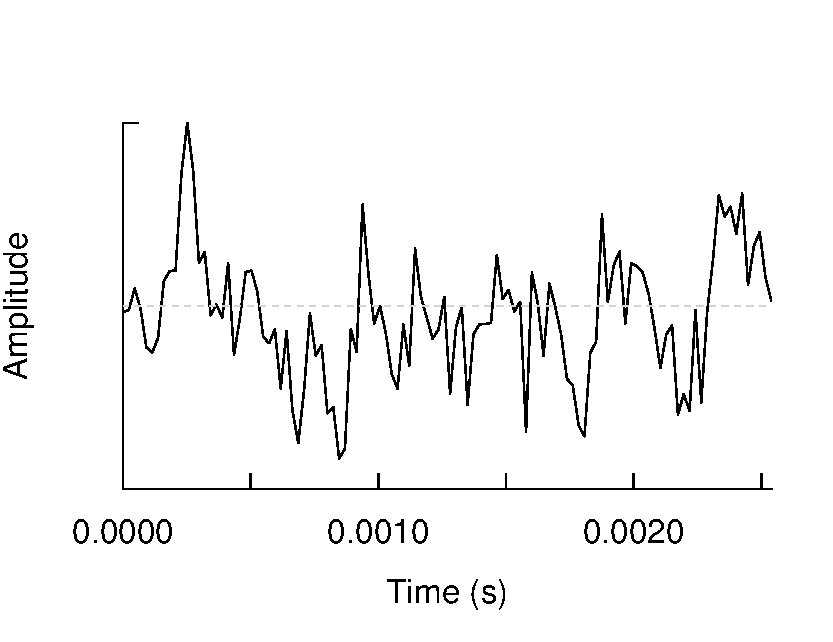
\includegraphics[height=192pt]{figures/pink_audio.pdf}}
\end{figure}

However, the time domain is not specifically bound to time intervals only. A
less intuitive, but realistic approach would be to model amplitude in the time
domain. That way the frequency relation to amplitude of a signal can be
analysed, but the time information is lost.

\subsection{Discrete wavelet transformation}
To be able to analyse and compare different wavelets, we need a way to scale
the signal. Discrete wavelet transformation is the operation of applying a
filter function, or set of filter functions (i.e., filter bank) to the wavelet.
This is a way of sampling the signal at different intervals giving a natural
means of scaling the signal \cite{karus2013}.

\paragraph{}
Wavelet analysis is similar to Fourier analysis with the difference that
wavelets deal with time and frequency information, and Fourier transform deals
with frequency information only. Wavelet analysis is the analysis of signals
(time-series) by decomposing the signal into wavelet/shift\footnote{Shifting,
or translating, is the operation of moving the wavelet in the time domain.}
coefficients and scaling/filter\footnote{Filtering, or dilating, is the
operation of scaling the wavelet in the frequency domain.} coefficients based
on wavelet functions (e.g., filters) \cite{karus2013}. The decomposition can be
repeated on the scaling/filter coefficients until the number of resulting
wavelet/shift coefficients is smaller than the filter length. The filter length
is a property of the filter function being used.

\paragraph{}
Wavelet transform has proven important in signal processing thanks to its
inherent properties which allow comparisons at different scales and shifts.
Compared to other time series analysis techniques, the main advantages of
wavelet transformations in the analysis of signals are \cite{karus2013}:
\begin{itemize}
	\item Wavelet/shift coefficients allow fuzzy matching as differences in details
	are 'smoothed out'.
	\item Filter/scale coefficients allow detection of small anomalies in series.
	\item Transform levels make series of different lengths or scale comparable.
\end{itemize}

\subsection{Wavelet functions}
A wavelet function is a function that defines a wavelet. In general, a wavelet
function is any operation on an existing wavelet \cite{wadkar}. Many wavelet
functions exist and differ largely in complexity and applicability depending on
the signal of interest.

A wavelet can be defined in the following ways, given that $T$ is the set of
time values of the signal, and $F$ the set of frequency values of the signal.
\begin{description}
	\item[Wavelet function (mother wavelet)] \hfill \\ $\Psi: T \rightarrow
	F$\\ $\Psi(t) = f$, such that $t \in T$ and $f \in F$.\\
	This function maps $T$ onto $F$ and thus produces the shape of the wavelet.

	\item[Scaling function (father wavelet)] \hfill \\ $\Phi: F \rightarrow
	T$\\ $\Phi(f) = t$, such that $t \in T$ and $f \in F$.\\
	This function maps $F$ onto $T$ and thus produces the scale of the wavelet.

	\item[Scaling filter] \hfill \\ A low-pass filter of length $2N$ and sum 1. A
	high-pass filter can be calculated as the quadrature mirror filter of the
	low-pass filter. Daubechies wavelets can be defined by the scaling filter.
\end{description}

\subsection{Haar wavelet}
The Haar wavelet is a member of the Daubechies family of wavelets, based on the
work of the Belgian mathematician Ingrid Daubechies. The Daubechies wavelets is
a family of orthogonal wavelets defining a discrete wavelet transform. All
wavelets of the Daubechies family can be entirely defined by their scaling
filter. The Haar wavelet has a filter of length 2 and is therefore also
referenced to as the Daubechies-2 (D2) filter. It is the simplest wavelet of
the Daubechies family.

\paragraph{}
In 1910, the Hungarian mathematician Alfred Haar introduced Haar functions. The
Haar transform is one of the earliest examples of what is known now as a
compact, dyadic, orthonormal wavelet transform \cite{stankovic}. The Haar
function is the simplest and oldest orthonormal wavelet with compact support.

\subsection{Discrete wavelet transformation using the Haar filter}
In each decomposition (e.g., each scaling or filtering step) the Haar function
adds more detail to the wavelets in the current level. The Haar filter captures
the differences between scale levels. The decomposition will be repeated until
the wavelets can no longer be divided. This happens when there is no more time
and/or frequency resolution left in the input signal to add further detail from
that signal.

\paragraph{}
Wavelet transformation using the Haar filter is widely used. For example, as a
way of digitalising an analogue signal in A-D converters, pattern recognition,
face recognition, image processing, data coding, multiplexing, digital
filtering, digital speech processing, voice controlled computing devices,
robotics, and compression mechanisms.

\begin{comment}
This chapter contains all the information needed to put the thesis into
context. It is common to use (a revised version) of your literature survey for
this purpose.
It is important to refer from your text to sources you have used, as listed in
your bibliography section (appendix). For example, “XP is a recent agile
development method [1]” is a common style of doing this, where the following
entry would be included in your bibliography:
[1] K. Beck, E. Gamma, Test infected: Programmers love writing tests, Java
Report 3 (7) (1998) 51–56.
If you want to refer to books you have read as part of the curriculum, you can
also do so in this way.
Have a look at Chapter 2 of this example thesis at Paul’s
homepage\footnote{http://homepages.cwi.nl/~paulk/thesesMasterSoftwareEngineering/2006/RichardKettelerij.pdf}.
\end{comment}
\chapter{Research}
Bla bla.
\chapter{Results}
\label{results}

\section{Data}
The data set of 250 projects was gathered in July 2013. It contains monthly
data points for each project up to June 2013.

The data set was tested for representativeness using the tool by
\citet{nagappan}. The data set scored a 99.5\% representativeness to the tool's
master data of 20,028 projects tracked by Ohloh.

\paragraph{}
The final data set contains monthly evolution data of 250 distinct projects
having a total of 22,943 data points. The oldest project having 321 monthly
data points, the youngest having 14 monthly data points. The first data point
in the set is of October 1986.

\section{Dead projects}
\label{section:deads}
A total of 38 (15.2\%) projects complied to the definition of a dead project as
defined in section \ref{def:dead}. Manual verification of the 38 potential
dead projects using the project's websites, source code repositories, and
commit history up to April 2014, revealed that 21 (8.4\%) are still complying
to the definition of a dead project in April 2014.

\paragraph{}
The 21 dead projects and their $age\_in\_months$ at the moment of death as a
result of the verification are shown in Table \ref{table:deads}.

\begin{wraptable}{l}{40mm}
\caption{Dead projects}\label{table:deads}
\centering
\begin{tabular}{rr}
  \hline
 ID & Died at month \\ 
  \hline
317799 &   2 \\ 
  587198 &   3 \\ 
  588411 &   5 \\ 
  589515 &   7 \\ 
  587204 &   8 \\ 
  585077 &   9 \\ 
  587571 &  11 \\ 
  586805 &  14 \\ 
  360279 &  30 \\ 
  322065 &  37 \\ 
  11389 &  46 \\ 
  12053 &  68 \\ 
  3085 &  71 \\ 
  307140 &  71 \\ 
  4614 &  75 \\ 
  41745 &  80 \\ 
  155830 &  84 \\ 
  325178 &  92 \\ 
  4007 & 120 \\ 
  15700 & 121 \\ 
  12547 & 142 \\  
   \hline
\end{tabular}
\end{wraptable}

\paragraph{}
All, except one, of the projects in Table \ref{table:deads} are dead because it
was abandoned by the community of contributors. Except for project \#587204,
which is still receiving updates, but at very slow and sporadic intervals.
However, since the updates do not involve code activity, it is considered dead.

\paragraph{}
When looking into project \#317799, which is the youngest in this set and died
in its second month, it shows that this project has had a history of the slightest
change in its lines of code evolution. The project has had a total number of 7
commits during the time it is being tracked by Ohloh (since September 2011). A
total of 4 contributors have worked on the project since it was tracked. The
most recent commit was done in October 2011.

\paragraph{}
Project \#12547 is the oldest. It died after 142 tracked months and has
had its most recent commits in February 2012. A total of 10 contributors have
worked on this project since May 2000.

\paragraph{}
The special case project \#587204, is the only project that is not
abandoned by its (entire) community. The project has had 3 contributors over its
lifetime. One of them is still active every now and then. The most recent
commits were done in January 2014, the commits before that were in June 2012.
The commits involved updates in documentation, and the creation of a
configuration file for a continuous integration server. These commits do not
involve code changes.

The project died in July 2012, after 8 months since the first data point
tracked.

\paragraph{}
From the initial 38 projects, the remaining 17 projects complying to the
definition of dead (section \ref{def:dead}) appeared to be still alive. These
17 projects are evaluated:

\begin{itemize}
	\item For 9 of the projects activity is very low or rapidly decreasing. Their
		community is slowly but surely abandoning the project as can be seen by a
		decrease of 35\% to 55\% of contributors, and/or commits.

	\item 5 of the projects are migrated to another source code repository. For
		these projects the tracking information is not updated at Ohloh and are lost.
		The tracking is stopped from the moment the project is migrated. The tracking
		and analysis can be recovered by updating the source code locations at Ohloh,
		but for this study the project is out of sight.

	\item The 3 projects that have had no activity in a year (i.e, were dead), but
		after that show little increase of activity are more difficult to explain.
		Manual evaluation showed that there exist similar projects outside the data
		set that eventually die, but there are also similar projects that eventually
		got 'resurrected'.
\end{itemize}



\section{Sequences and patterns}
\label{section:seqs_patterns}
The wavelet transform of the LOC signals of 250 projects resulted in 22,943
data points decomposed up to 7 levels into wavelet/shift and filter/scale
coefficients.

\begin{table}[H]
\caption{Similar sequences count}\label{table:sequence_counts}
\centering
\begin{tabular}{lrr}
\hline
	Total & 1,669,448 & 100.000\% \\
	\hline
	In filter/scale coefficients & 1,669,432 & 99.999\% \\
	In wavelet/shift coefficients & 16 & 0.001\% \\
\hline
\end{tabular}
\end{table}


\noindent
As shown in Table \ref{table:sequence_counts}, the similar sequence
identification found a total of 1,669,448 sequences that occurred at least 2
times. A mere 16 sequences were found in wavelet/shift coefficients, the other
1,669,432 sequences were found in filter/scale coefficients.

\paragraph{}
The second wavelet analysis step aggregated similar sequences across multiple
pairs together to form patterns. The detection of these 'popular sequences'
found 16,049 patterns. The patterns consist only of sequences of scale/filter
coefficients.

\paragraph{}
An arbitrary pattern that was found is shown in Figure
\ref{figure:patterns_plots}. The graph shows the similarity of the pattern with
its occurrences across multiple projects. Time is indexed and LOC is
represented as coefficients. This is due to the fact that wavelet transform
scales and filters these measures and thus no longer represent real-world
values such as months or actual lines of code.

\begin{figure}[H]
\caption{Example of a pattern found during wavelet
analysis}\label{figure:patterns_plots}
\centering
	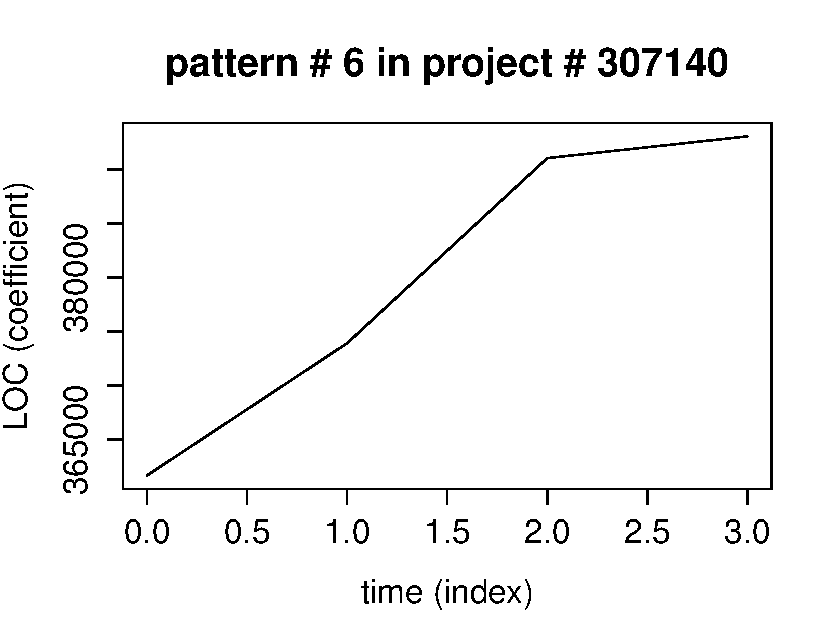
\includegraphics[width=196pt]{images/pattern_6.pdf}\\
	\vspace{1em}
	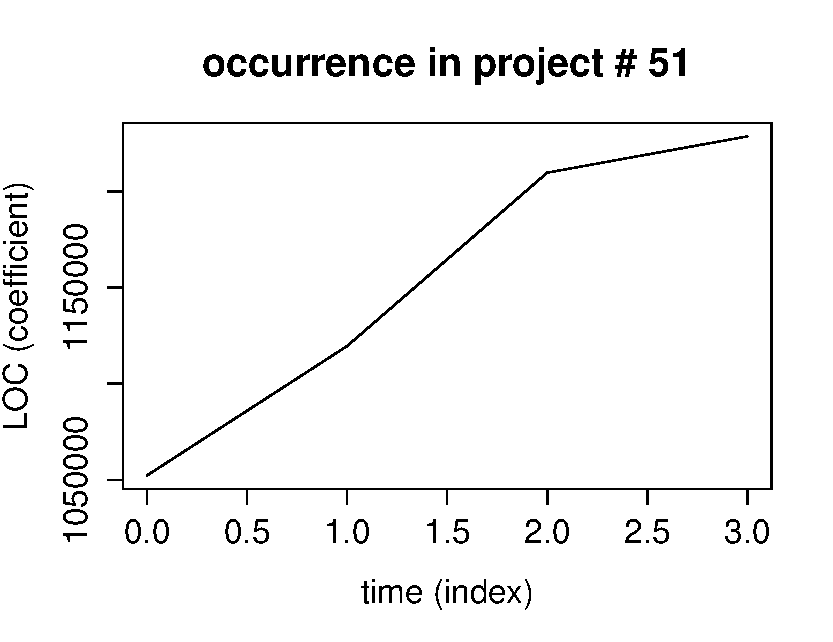
\includegraphics[width=128pt]{images/pattern_6_seq_e.pdf}
	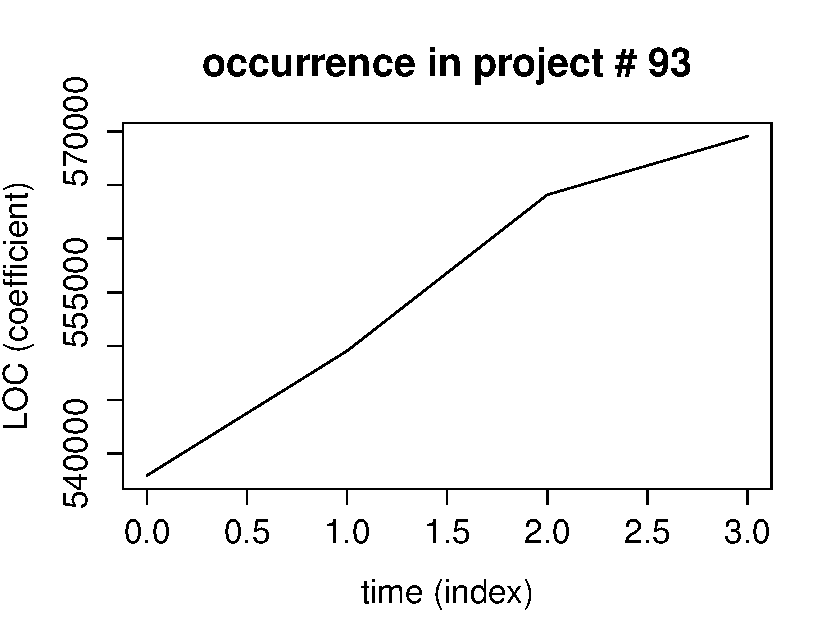
\includegraphics[width=128pt]{images/pattern_6_seq_d.pdf}
	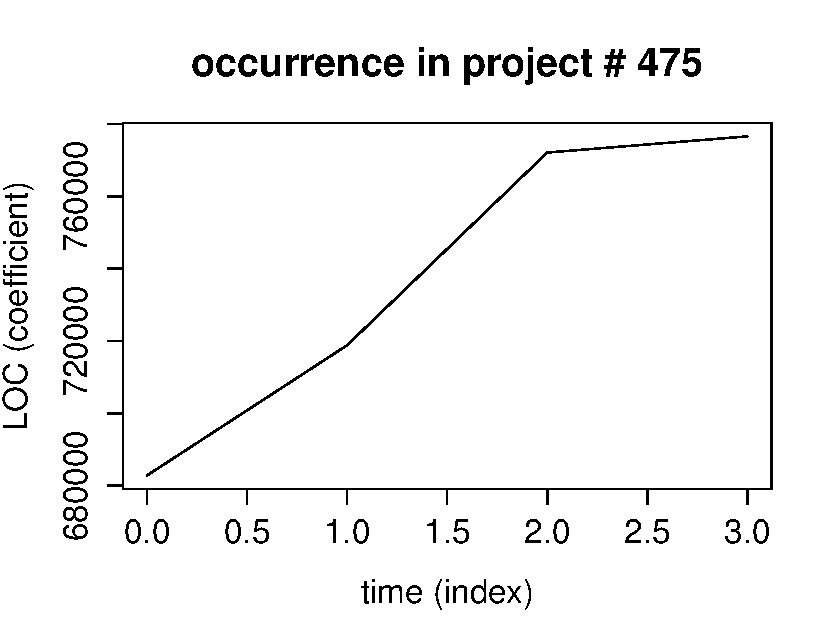
\includegraphics[width=128pt]{images/pattern_6_seq_c.pdf}
	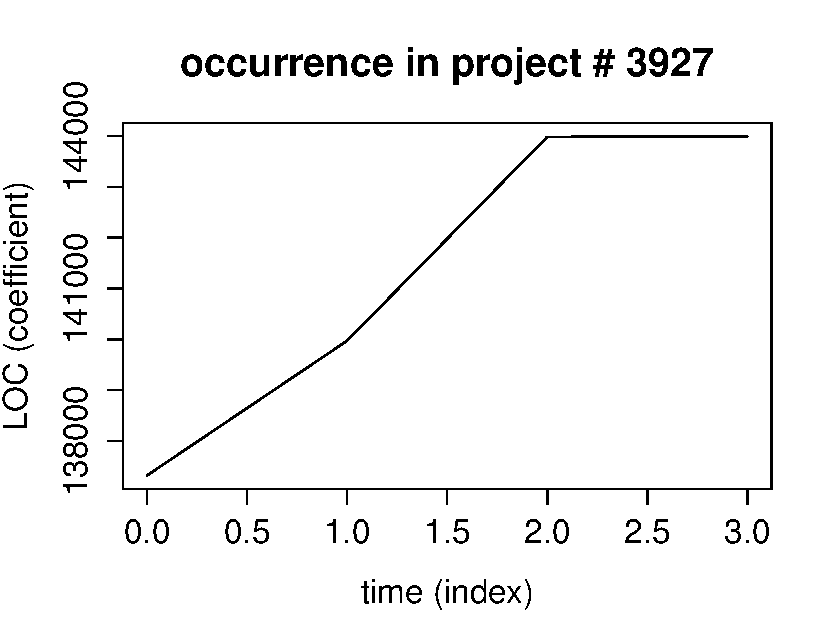
\includegraphics[width=128pt]{images/pattern_6_seq_f.pdf}
	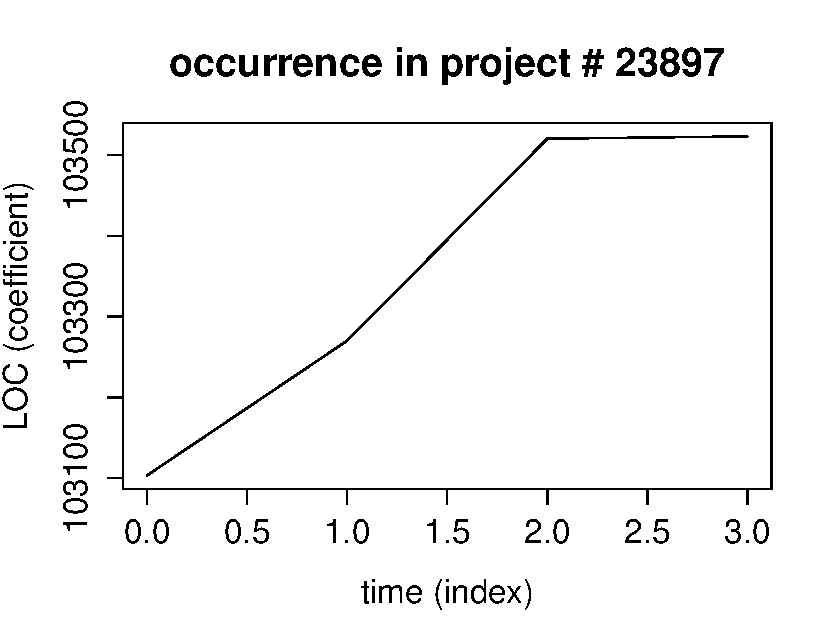
\includegraphics[width=128pt]{images/pattern_6_seq_a.pdf}
	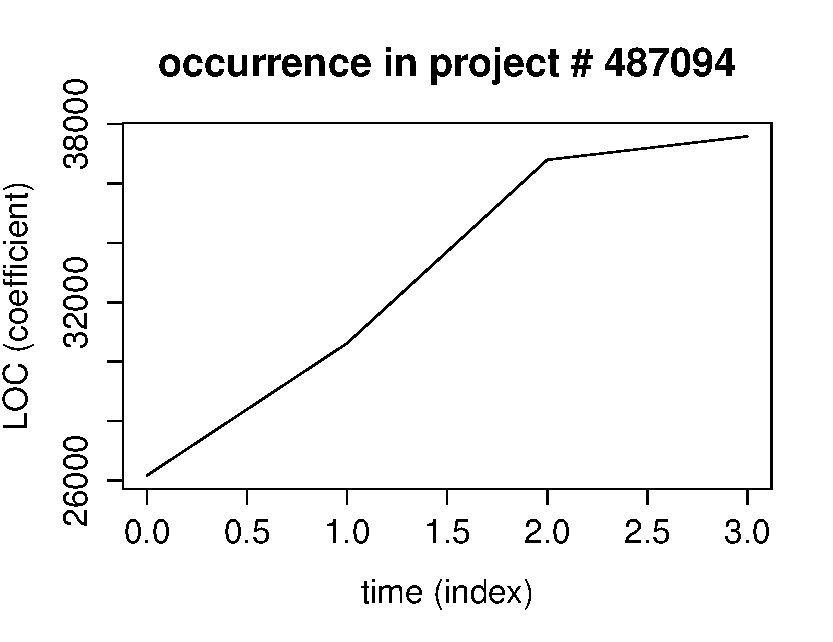
\includegraphics[width=128pt]{images/pattern_6_seq_b.pdf}
\end{figure}

\paragraph{}
The patterns occurred between 5 and 1,512 times across the projects. On
average, a pattern occurs 104 times. A single pattern occurs in at least 1 and
at most 204 projects (36 projects on average). The pattern length is between 4
and 19 coefficients (on average 6) across decomposition levels 3 to 7.

On the 3\textsuperscript{th} level, the average pattern length is equal to 4
coefficients. Every subsequent level doubles the average pattern length. This
is expected as there are twice as many coefficients available. This means the
same pattern is detected at multiple levels. Additionally, it can be said that
a pattern has multiple levels.

\paragraph{}
Table \ref{table:pattern_counts} presents the numbers of patterns
detected and occurring across projects. Recall the distinction between
detecting and occurring patterns from section \ref{def:pattern}.

\begin{table}[H]
\caption{Patterns detected and occurring}\label{table:pattern_counts}
\centering
\begin{tabular}{lrr|rr}
\hline
	\bfseries{Patterns detected}\rm & & & \bfseries{Count} \\
	\hline
	total & & & 16,049 & 100.00\% \\
	\hline
	in dead projects & & & 1,084 & 6.75\% \\
	in alive projects & & & 14,965 & 93.25\% \\
\hline\hline
	\bfseries{Patterns detected in dead projects}\rm & \bfseries{Occurrences}\rm
	& & \bfseries{Count}\rm \\
	\hline
	total & 111,848 & 100.00\% & 1,084 & 100.00\% \\
	\hline
	in dead projects only & 111 & 0.10\% & 16 & 1.48\% \\
	%in alive projects only & 0 & 0.00\% & 0 & 0.00\% \\
	in both dead and alive projects & 111,737 & 99.90\% & 1,068 & 98.52\% \\
\hline\hline
	\bfseries{Patterns detected in alive projects}\rm & \bfseries{Occurrences}\rm & & \bfseries{Count}\rm \\
	\hline
	total & 1,560,883 & 100.00\% & 14,965 & 100.00\% \\
	\hline
	%in dead projects only & 0 & 0.00\% & 0 & 0.00\% \\
	in alive projects only & 37,333 & 2.39\% & 3,390 & 22.65\% \\
	in both dead and alive projects & 1,523,550 & 97.61\% & 11,575 & 77.35\% \\
\hline
\end{tabular}
\end{table}

\noindent
As can be seen from Table \ref{table:pattern_counts}, 16,049 patterns were
detected across 250 projects, which is 64.2 patterns per project on average;
14,965 patterns were detected across 229 alive projects (65.3 patterns on
average per project); and 1,084 patterns detected in 21 dead projects (an
average of 51.6 patterns per project). The averages do not differ significantly
over the projects.



\section{Pattern classification}
The classification of the patterns was done to distinguish different types of
patterns to be able to find evolutionary events. For this, the patterns
detected in dead projects were taken and classified according to
the definitions in section \ref{section:patterns_dead}. It is expected that
this group has the highest chance of keeping a pattern indicating an
evolutionary event leading to the end of code evolution.

\paragraph{}
A total of 1,084 patterns detected in dead projects is classified. The sizes of
the pattern type subsets are shown in Table \ref{table:pattern_type_counts}.
For each subset, it is stated in how many projects a pattern of that type was
found.

\begin{table}[H]
\caption{Pattern types}\label{table:pattern_type_counts}
\centering
\begin{tabular}{rrr|rr}
\hline
	\bfseries{Type}\rm & \bfseries{Pattern count}\rm & & \bfseries{Occurrences}\rm
	& \bfseries{Project count}\rm \\
	\hline
	A & 13 & 1.20\% & 167 & 93 \\
	B & 382 & 35.24\% & 10,741 & 204 \\
	AB & 689 & 63.56\% & 100,967 & 226 \\
	\hline
	 & 1,084 & 100.00\% &  \\
\hline
\end{tabular}
\end{table}


\section{Survivability}
As described in section \ref{section:survivability}, the survivability of the
projects having a type A pattern is estimated.

The groups G0 -- projects without an occurrence of a type A pattern --, and G1
-- the projects having an occurrence of a type A pattern -- both contain 93
projects. Projects in G1 are selected by the characteristic of the occurrence
of a type A pattern. This comprises 93 different projects as can be seen in
Table \ref{table:pattern_type_counts}. The projects for the control group G0
are selected as not occurring in G1 and being representative to the whole set
of 250 projects.

\subsection{Group G0}
\label{section:group_g0}
The four projects in group G0 that die are shown in Table \ref{table:deads_g0}.
As stated in section \ref{section:deads}, all dead projects except \#587204 are
abandoned by their communities.

\begin{table}[H]
\caption{Dead projects in G0}\label{table:deads_g0}
\centering
\begin{tabular}{rrll}
\hline
	\textbf{Project} & \textbf{Final age} & \textbf{Reason} & \textbf{Patterns
	found} \\
	\hline
	587198 & 3 & Abandoned & AB only (9) \\
	588411 & 5 & Abandoned & AB only (12) \\
	587204 & 8 & Non-code activity & AB (15), B (4) \\
	586805 & 14 & Abandoned & AB (6), B (1) \\
\hline
\end{tabular}
\end{table}

\noindent
Table \ref{table:deads_g0} shows that the four dead projects of group G0 have
no pattern of type A, which is true by the definition of the group. However,
they do all have occurrences of patterns of type AB. This means that there are
patterns detected in these four projects that occur near and last until the end
of code evolution of these projects. Further evaluation shows that the 42 AB
patterns from these four projects all show a stagnation in LOC change. The
difficulty is that the type AB patterns also occur somewhere else in a dead
project's evolution, which makes it hard by current definitions to identify as
possible warning signs.

\paragraph{}
The other 89 projects of G0 stay alive. Their age varies between 13 and 255
months.

\subsection{Group G1}
\label{section:group_g1}
The dead projects in group G1 are shown in Table \ref{table:deads_g1}. The
column 'TTL' ('time to live') states the number of months the project has
lived between the 'diagnosis' of the type A pattern and the death of the
project. The 'Diagnosed' column states the age in months the pattern was found.

\begin{table}[H]
\newcommand{\tableDeadsGOneHead}{\textbf{Project} & \textbf{Final age} &
\textbf{TTL} & \textbf{Diagnosed}}
\caption{Dead projects in group G1}\label{table:deads_g1}
\centering
\begin{tabular}{rrrr}
\hline
	\tableDeadsGOneHead\\
	\hline
	3085 & 71 & 20 & 51 \\
	4007 & 120 & 36 & 84 \\
	4614 & 75 & 22 & 53 \\
	11389 & 46 & 37 & 9 \\
	12053 & 68 & 13 & 55 \\
	15700 & 121 & 120 & 1 \\
	41745 & 80 & 22 & 58 \\
\hline
\end{tabular}
\hspace{1em}
\begin{tabular}{rrrr}
\hline
	\tableDeadsGOneHead\\
	\hline
	155830 & 84 & 41 & 43 \\
	307140 & 71 & 70 & 1 \\
	317799 & 2 & 1 & 1 \\
	322065 & 37 & 30 & 7 \\
	325178 & 92 & 4 & 88 \\
	360279 & 30 & 1 & 29 \\
	587571 & 11 & 8 & 3 \\
\hline
\end{tabular}
\end{table}

\noindent
All projects in Table \ref{table:deads_g1} are abandoned (see section
\ref{section:deads}). One quarter of the projects in the table live 9 months
after a type A pattern was found. Another quarter lives 36 months after
diagnosis. The dead projects in group G1 on average live up to 30 months since
a type A pattern was found.

Project \#15700 is an outlier; an occurrence of a type A pattern was found when
the project was 1 month old, but it lived for another 10 years before it died.

\paragraph{}
The majority (79) of the projects in group G1 are still alive. The 75 projects
that have been 'diagnosed' of a type A pattern have had the occurrence in their
first month of age. Only in 4 projects the pattern was found later: 23, 33, 52
and 62 months.

\subsection{Estimation of survival}
The Kaplan-Meier estimation of survival function for the projects is shown in
Figure \ref{figure:kp_survival}, having the survival probability on the
vertical axis, and the age in months of projects on the horizontal axis.

The numbers at the bottom, divided in two rows representing group 0 and group
1, represent the number of projects alive per group at the corresponding point
on the horizontal axis.

\begin{figure}[H]
\caption{Kaplan-Meier estimation survival of projects regarding type A
patterns}\label{figure:kp_survival}
\centering
	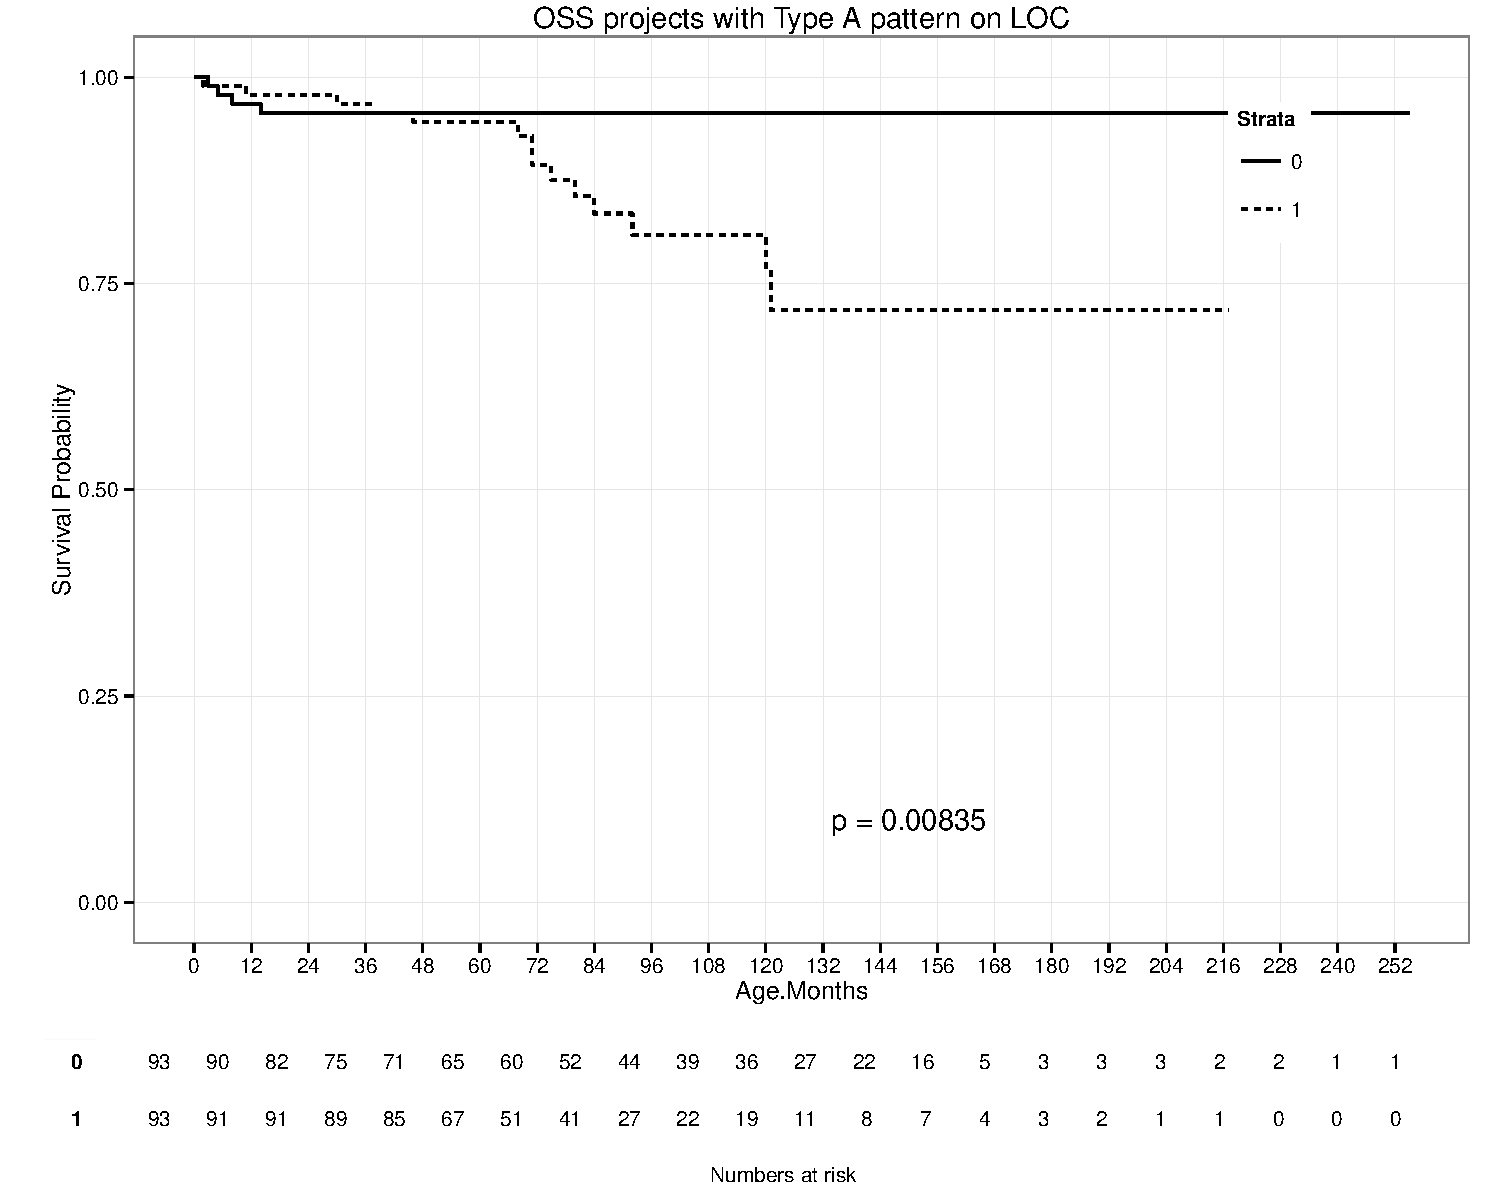
\includegraphics[width=386pt]{images/survival_LOC.pdf}
\end{figure}

\noindent
The Kaplan-Meier estimation of the survival function of the projects as shown
in Figure \ref{figure:kp_survival} visualise the survival probability of
the projects with and without the occurrence of a type A pattern.

The figure shows a p-value of $p = 0.00835$. This is the log-rank value
representing the comparability of the two groups. In general, a p-value of $p >
0.05$ indicates the two groups are incomparable (i.e., the two groups do not
show significant differences). Thus, the p-value of $p = 0.00835$ indicates
comparable groups. Typically, the larger the groups, the lower the p-value.
It seems a group size of 93 projects is large enough to estimate survivability
of projects having an occurrence of a type A pattern.

\paragraph{}
The groups do not contain censored projects, i.e., there are no projects
lost to follow-up. This increases the reliability of the estimation because all
projects in are either dead or alive at any point in the curve (i.e., they are
all 'at risk' of dying).

\paragraph{}
Figure \ref{figure:kp_survival} shows that the projects of G0 have a survival
chance of approximately 93\% after the first year. In the first 12 months, the
survival chances drop to around 86\%. After that, the survival chance remains
stable for projects in G0.

More than half of the projects in G0 lives longer than 84 months (7 years)
against 72 months (6 years) in G1. A quarter of the projects in G0 lives longer
than 144 months (12 years), against 108 months (9 years) in G1. Two projects of
G0 outlives all projects in G1 after 18 years.

\paragraph{}
During the first year, the projects of G1 have 3\% higher survival chance than
those of G0: approximately 96\%. It is after 4 years that the projects of G1
have a lower survival chance than those in G0. Between approximately 3.2 and
3.8 years of age, projects in both groups show equal survival chances.

\begin{comment}
- Factual results
- Tables and figures for clarification

This chapter presents and clarifies the results obtained during the research.
The focus should be on the factual results, not the interpretation or
discussion. Tables and graphics should be used to increase the clarity of the
results where applicable.
Have a look at the the results chapter in this example thesis on Paul’s
homepage\footnote{http://homepages.cwi.nl/~paulk/thesesMasterSoftwareEngineering/2006/ArnoldLankamp.pdf}.
\end{comment}

\chapter{Analysis and Conclusions}
\label{analysis}

% answer subquestion one: what patterns can be found using wavelet analysis?
\section{Sequence analysis}
There are more than 100,000 times more similar sequences found in the
scale/filter coefficients than in the wavelet/shift coefficients. The large
difference in number of sequences found between the two types of coefficients
is due to the fact that the LOC metric is a cumulative metric. The typical shape
of the LOC metric is a growing line. This makes finding a matching sequence of
coefficients using only shift coefficients (i.e., along the time axis) less
likely.

\paragraph{}
The fact that, of the 16,049 patterns, there are 0 patterns found in shift
coefficients was to be expected. The 16 similar sequences in shift coefficients
are not similar within the same group of sequences. Additionally, the shift
coefficients are incomparable to the filter coefficients because it is a
fundamentally different way of signal transformation. Mixing both types of
coefficients would ignore how the coefficients were found and invalidate the
patterns.

\section{Pattern evaluation}
\label{section:pattern_evaluation}
To be able to know what the patterns represent, the 16,049 patterns are
projected onto the original signal. This is done by finding the project the
pattern was first detected, and taking the pattern's level of decomposition and
starting point in the series of coefficients for its project.

As the set of values of level of decomposition, starting point in the series,
its length (i.e., number of coefficients), and the originating project is
unique for each pattern, it can be 're-projected' onto the signal of that
particular project. This gives the $age\_in\_months$ values the sequence starts
and ends in the project.

Knowing the start and end month of a sequence within a project, the values of
the original signal during the sequence are captured for further analysis.

\paragraph{}
The absolute maximum differences of the LOC values is computed for each
sequence. The patterns have maximum LOC differences between 0 (i.e., no change
in LOC in the sequence) and 6,862,111. Figure \ref{figure:pattern_loc_diff}
shows the distribution of this number across the patterns.

\begin{figure}[H]
\caption{Distribution of maximum LOC differences across
patterns}\label{figure:pattern_loc_diff}
\centering
	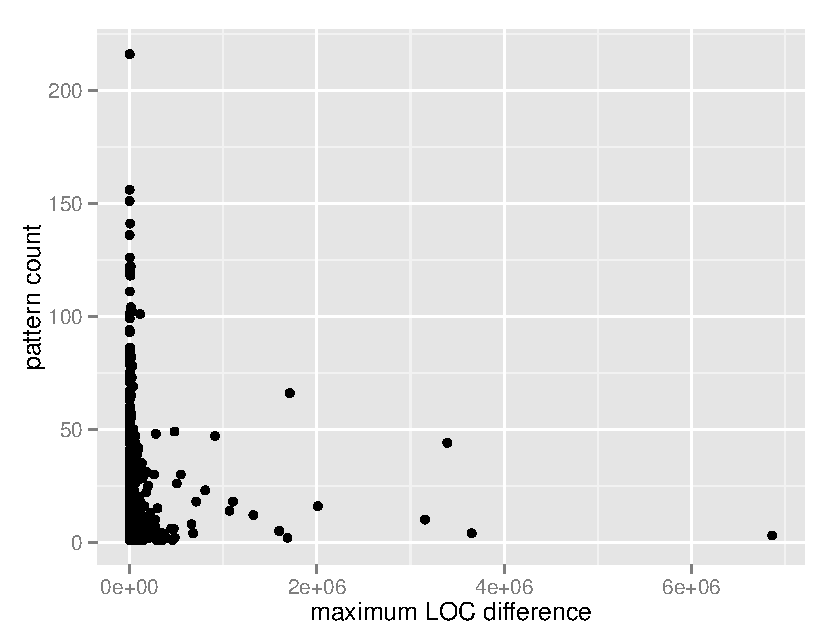
\includegraphics[width=296pt]{images/pattern_LOC_diff_100.pdf}
\end{figure}

75\% of the patterns have a maximum LOC difference less than 20,595; 50\% have
a maximum LOC difference less than 5,250; and 25\% less than 1,046.

\paragraph{}
The top four patterns with least maximum LOC differences are shown in Figure
\ref{figure:top_patterns_plots} to illustrate how such patterns look like. The
figure depicts the wavelets of the patterns for all the project signals they
were detected in. Which are the differences in LOC values between two subsequent
coefficients.

The graphs show that the sequences have similar waveforms. Each graph contains
a multiple of plotted sequences: pattern 1: 216 sequences; pattern 2: 156
sequences; pattern 3: 151 sequences; and pattern 4: 141 sequences. Note that
the factor of scale is reintroduced, because the sequences all contain
scale/filter coefficients. The factor of time, however, is still being
eliminated, hence the use of \emph{index }\rm instead of a time metric on the
horizontal axis.

\begin{figure}[H]
\caption{The four most common type A patterns projected onto original
signal}\label{figure:top_patterns_plots}
\centering
	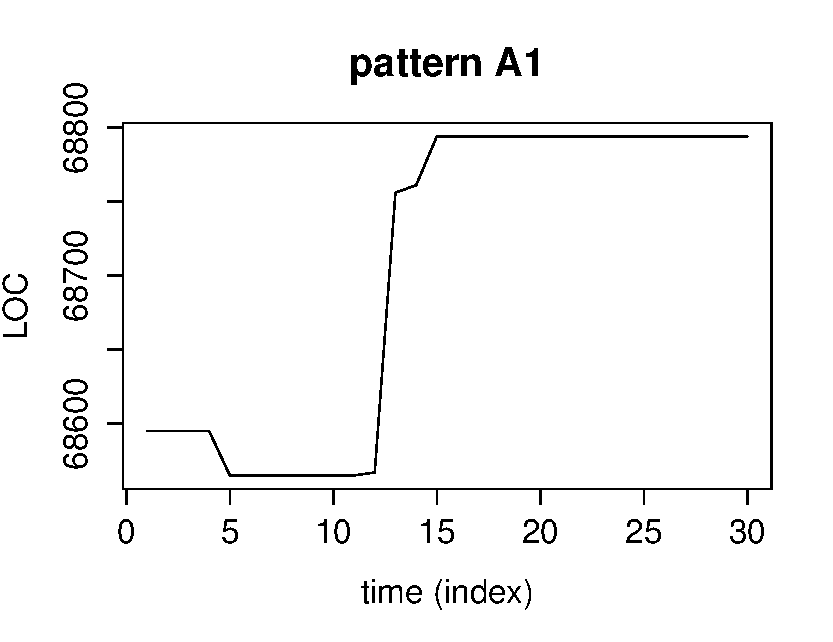
\includegraphics[width=196pt]{images/pattern_a1.pdf}
	\hspace{1em}
	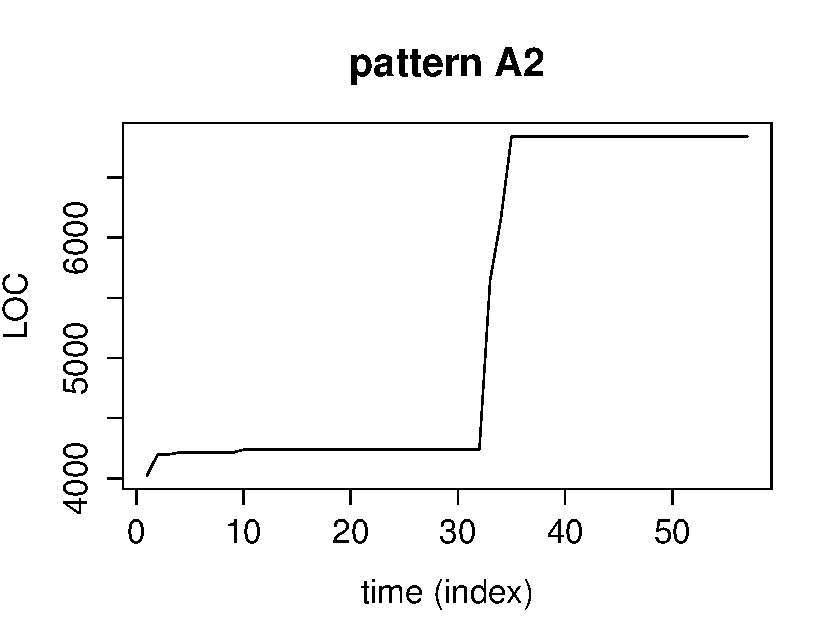
\includegraphics[width=196pt]{images/pattern_a2.pdf}
	\\
	\vspace{1em}
	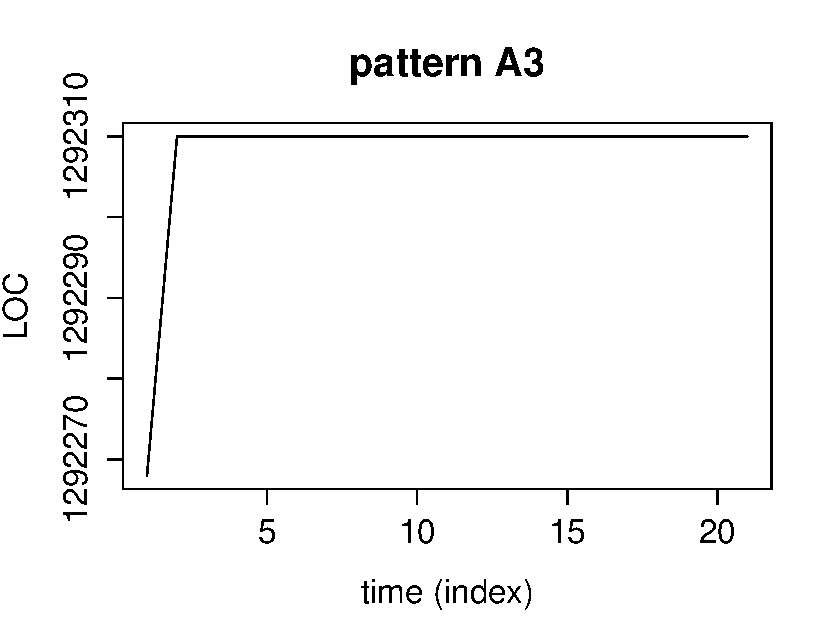
\includegraphics[width=196pt]{images/pattern_a3.pdf}
	\hspace{1em}
	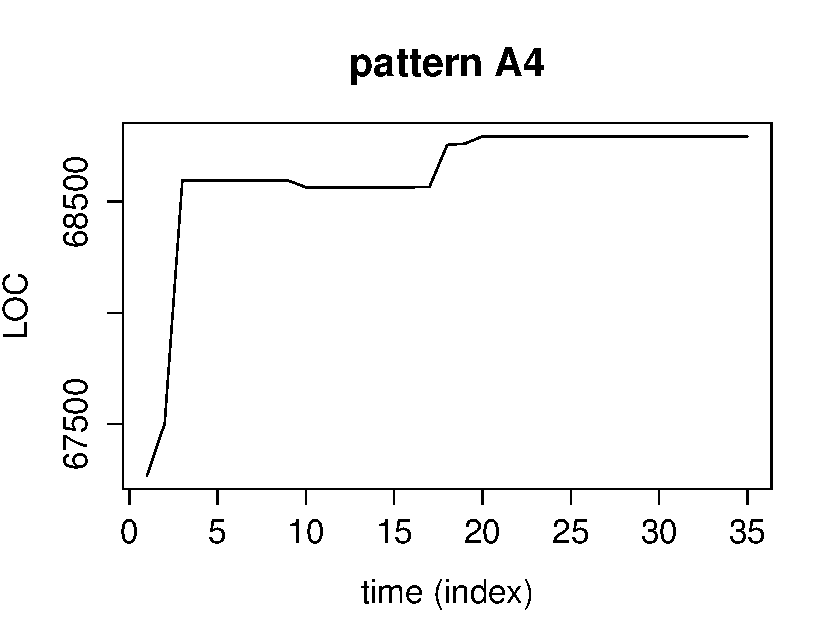
\includegraphics[width=196pt]{images/pattern_a4.pdf}
\end{figure}

\section{Conclusions}
%Many more sequences were found using filtering. This is expected as scaling is
% better than shifting at finding small coefficients.

\section{Threats to validity}
\begin{comment}
* Is the Ohloh database a representation of the world of OSS projects?
* Is LOC as the sum of source lines of code, comments, and blank lines valid?
* The use of LOC as a measure of project evolution. Does it represent
activity/growth/whatever to say something about the project's status?
* A selection criterion for the projects was a continuous series of subsequent
monthly facts. Maybe the full series of evolution data of a project is needed in
order to find objective signs or to be able to compare different projects.
* Is 250 projects enough to detect patterns and generalise to the world of OSS
projects?
* Is monthly aggregated data fine-grained enough?

\end{comment}

\section{Future work}


\begin{comment}
- Analyse results
- Conclude and interpret results
- Answer research questions
- Threats to validity
- Discussion
- Future work
 
This chapter contains the analysis and interpretation of the results. The
research questions are answered as best as possible given the results that were
obtained. The analysis also discussed parts of the questions that were left
unanswered.

An important topic is the validity of the results.
What methods of validation were used?
Could the results be generalized to other cases?
What threats to validity can be identified?

There is room here to discuss the results of related scientific literature here
as well.
How do the results obtained here relate to other work, and what consequences are
there?
Did your approach work better or worse?
Did you learn anything new compared to the already existing body of knowledge?
Finally, what could you say in hindsight on the research approach by followed?
What could have done better?
What lessons have been learned?
What could other researchers use from your experience?

A separate section should be devoted to ‘future work,’ i.e., possible extension
points of your work that you have identified. Other researchers (or yourself)
could use those as a starting point.

Refer to Chapters 3.7 and 4 in this example thesis at Paul’s
homepage\footnote{http://homepages.cwi.nl/~paulk/thesesMasterSoftwareEngineering/2006/ReneWiegers.pdf}.
\end{comment}


\bibliography{thesis}{}
\bibliographystyle{myplainnat}

%% appendices

%\cleardoublepage
%\listoffigures
%\phantomsection
%\addcontentsline{toc}{chapter}{\listfigurename}

\cleardoublepage
\listoftables
\phantomsection
\addcontentsline{toc}{chapter}{\listtablename}

\end{document}
